\section{Defining five equivalence classes}
\label{sec:equivClasses}

\subsection{Conceptual Overview}
This chapter introduces possible refactorings in regular expressions by identifying equivalence classes of Python Regular Expressions, identifying what representations are possible in each equivalence class, and also identifying what transformations between representations are possible. As with source code, in regular expressions there are often multiple ways to express the same semantic concept.
For example, \cverb!AAA*! matches two \verb!`A'!s followed by zero or more \verb!`A'!s.  This matching behavior is identical to the behavior of the syntactically different regex \cverb!AA+!, which matches two or more \verb!`A'!s.  What is not clear is which representation,  \cverb!AAA*!  or  \cverb!AA+!, is preferred.

Preferences in regular expression refactorings could come from a number of sources, including which is easier to maintain, easier to understand, or better conforms to community standards, depending on the goals of the programmer.  By investigating which representation appears most frequently in source code, we can establish a community standard and suggest refactorings based on conformance to that standard.


\begin{figure*}[tb]
\centering
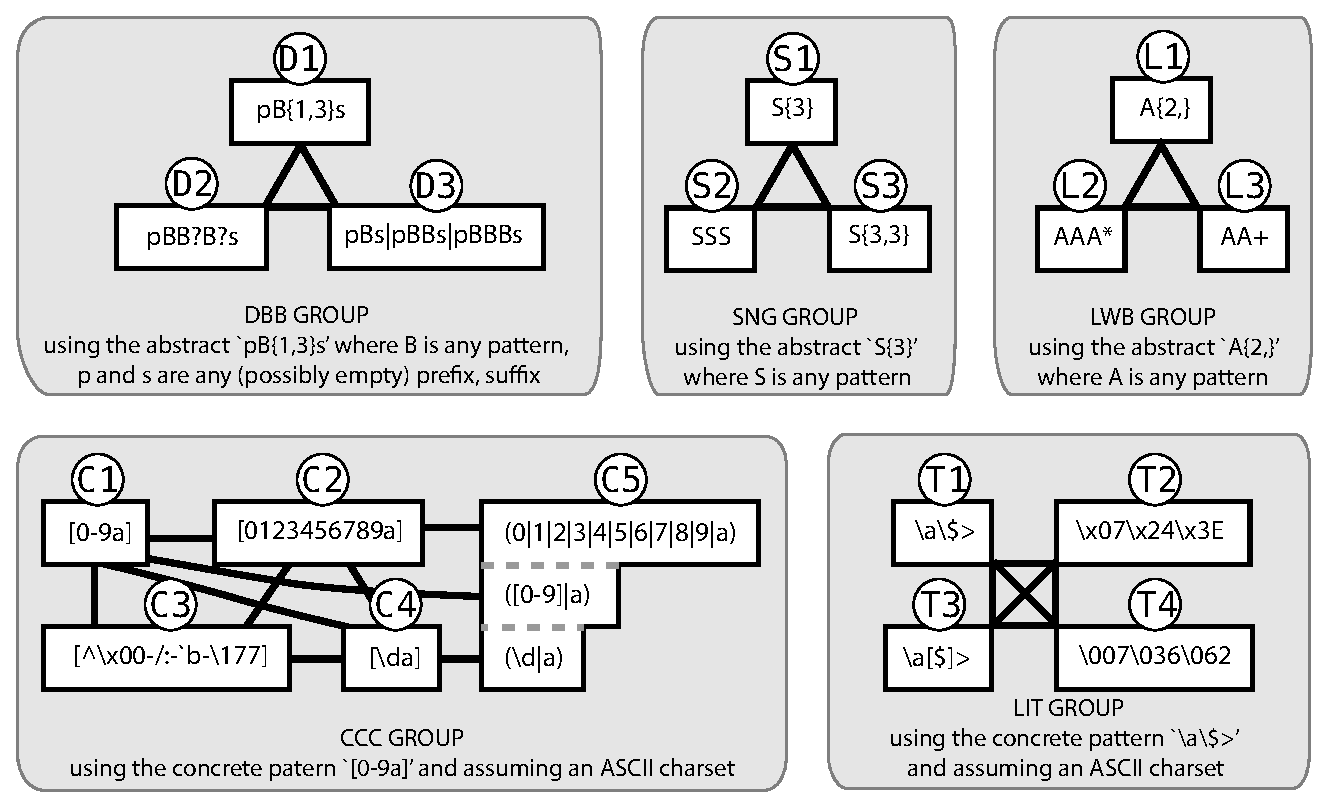
\includegraphics[width=\textwidth]{nontex/illustrations/refactoringTree.eps}
\vspace{-12pt}
\caption{Equivalence classes with various representations of semantically equivalent representations within each class. DBB = Double-Bounded, SNG = Single Bounded, LWB = Lower Bounded, CCC = Custom Character Class and LIT = Literal}
\vspace{-6pt}
\label{fig:refactoringTree}
\end{figure*}

Figure~\ref{fig:refactoringTree} displays five equivalence classes in grey boxes.  These equivalence classes provide options for how to represent double-bounds in repetitions (e.g., \cverb!a{1,2}! or \cverb!a|aa!), single-bounds in repetitions (e.g., \cverb!a{2}! or \cverb!aa!), lower bounds in repetitions (e.g., \cverb!a{2,}! or \cverb!aaa*!), character classes (e.g., \cverb![0-9]! or \cverb![\d]!), and literals (e.g., \cverb!\a! or \cverb!\x07!).  This work will often use the term \emph{group} as shorthand for `equivalence class'.

Each equivalence class has multiple \emph{nodes} which each represent different ways to express or \emph{represent} the behavior of a particular regex.  Examples of various semantically equivalent \emph{representations} of a regex are shown in white boxes. A \emph{representation} is a particular regex that expresses matching behavior using the style of a particular \emph{node}.

As an example of one equivalence class, consider the LWB group.  Each node in the LWB group has a lower bound on repetitions. Regexes \cverb!A{2,}!, \cverb!AAA*! and \cverb!AA+! are semantically equivalent regexes belonging to the nodes L1, L2 and L3, respectively.
The undirected edges between nodes define possible refactorings.
Identifying the best direction for each arrow in the possible refactorings is discussed in Section~\ref{sec:ordering}.

Figure~\ref{fig:refactoringTree} uses specific examples to more clearly illustrate the characteristics of each node.  However, the \verb!`A'!s in the LWB group abstractly represent any element, and the number of elements is free to vary. We chose the lower bound repetition threshold of 2 for illustration; in practice this could be any number, including zero.
Next, we describe the characteristics of all nodes of each group in detail:

\subsection{CCC Group}
The Custom Character Class (CCC) group contains five nodes that each require the expression of a set of characters, as is typical when using the CCC feature.  For example, the regex \cverb!b[ea]t! will match both \verb!"bet"! and \verb!"bat"! because, between the \verb!`b'! and \verb!`t'!, the CCC \cverb![ae]! specifies that either \verb!`a'! or \verb!`e'! (but not both) must be present.
We use the term \emph{custom} to differentiate these classes created by the user from the default character classes: \cverb!\d!, \cverb!\D!, \cverb!\w!, \cverb!\W!, \cverb!\s!, \cverb!\S! and \cverb!.! provided in Python Regular Expressions.
Next, we provide descriptions of each node in this equivalence class:

\begin{description}  \itemsep -1pt
\item[C1:] Any regex using the RNG feature in a CCC like \cverb![a-f]! as shorthand for all of the characters between \verb!`a'! and \verb!`f'! (inclusive) belongs to the C1 node.  C1 does \emph{not} include any regex using the NCCC feature.  All regex containing NCCC belong to the C3 node.

\item[C2:] Any regex that contains at least one CCC without any RNG or defaults belongs to the C2 node. For example, \cverb![012]! is in C2 because it does not use any RNG or defaults, but \cverb![0-2]! is not in C2 because it uses RNG.  Similarly, \cverb![Q\d]! is not in C2 because it uses the DEC default character class.  Membership to C2 only requires one CCC without RNG or defaults, so \cverb![abc][0-9\s]! \emph{does} belong to C2 because it contains \cverb![abc]!.

\item[C3:] Any regex using the NCCC feature belongs to the C3 node.  For example \cverb![^ao]! belongs to C3, and \cverb![ao]! does not (notice the \verb!`^'! character after the \verb!`['!).

For a given charset (e.g., ASCII, UTF-8, etc.), any CCC can be represented as an NCCC.  Consider if the PRE engine was using an ASCII charset containing only the following 128 characters: \verb!\x00-\x7f!.  Consider that a CCC representing the lower half: \cverb![\x00-\x3f]! can be represented by negating the upper half: \cverb![^\x40-\x7f]!.

\item[C4:] Any regex using a default character class in a CCC like \cverb![\d]! or \cverb![\W]! belongs to the C4 node.

\item[C5:] Any regex containing an OR of length-one sequences (including defaults or other CCCs) belongs to the C5 node.  These representations can be transformed into a CCC syntax by removing the OR operators and adding square brackets.  For example \cverb!(\d|a)! in C5 is equivalent to \cverb![\da]! in C4.

Because an OR cannot be directly negated, it does not make sense to have an edge between C3 and C5 in Figure~\ref{fig:refactoringTree}, though C3 may be able to transition to C1, C2 or C4 first and then to C5.
\end{description}

A regex can belong to multiple nodes of the CCC group. For example, \cverb![a-f\d]! belongs to both C1 and C4.  The edge between C1 and C4 represents the opportunity to express the same regex as \cverb![a-f0-9]! by transforming the default digit character class into a range.  This transformed version would only belong to the C1 node.  Not all regexes in C1 contain a default character class that can be factored out.  For example \cverb![a-f]! belongs to C1 but cannot be transformed to an equivalent representation belonging to C4.

\subsection{DBB Group}
The double-bounded (DBB) group contains all regexes that use some repetition defined by a (non equal) lower and upper boundary.  For example the regex \cverb!pB{1,3}s! requires one \verb!`p'! followed by one to three sequential \verb!`B'!s, then followed by a single \verb!`s'!.  This regex will match \verb!"pBs"!, \verb!"pBBs"!, and \verb!"pBBBs"!.

\begin{description}  \itemsep -1pt
\item[D1:] Any regex that uses the DBB feature (curly brace repetition with a different lower and upper bound), such as \cverb!pB{1,3}s!, belongs to the D1 node.

Note that \cverb!pB{1,3}s! can become \cverb!pBB{0,2}s! by pulling the lower bound out of the curly braces and into the explicit sequence (or visa versa). Nonetheless, it would still be part of D1, though this within-node refactoring on D1 is not discussed in this work.
\item[D2:] Any regex that uses the QST feature (a question mark indicating zero-or-one repetition) belongs to D2. An example regex belonging to D2 is \cverb!zz?!, which matches \verb!"z"! and \verb!"zz"!.

When a regex belonging to D1 has zero as the lower bound, it can be transformed to a representation belonging to D2 by replacing the DBB feature and the element it operates on (like the \cverb!B{0,2}! in \cverb!pBB{0,2}s!) with $n$ new regexes composed of the element operated on by DBB followed by QST, where $n$ is equal to the upper bound in the DBB.  For example \cverb!B{0,2}! has a zero lower bound and an upper bound of 2, so it can be represented as \cverb!B?B?!.  Therefore \cverb!pBB{0,2}s! can become \cverb!pBB?B?s!.
\item[D3:] Any regex that uses OR to express repetition with different upper and lower boundaries like \cverb!pBs|pBBs|pBBBs! belongs to D3.  The example \cverb!pB{1,3}s! becomes \cverb!pBs|pBBs|pBBBs! by explicitly stating the entire set of strings matched by the regex in an OR.
\end{description}

Note that a regex can belong to multiple nodes in the DBB group, for example, \cverb!(a|aa)X?Y{2,4}! belongs to all three nodes: \cverb!Y{2,4}! maps it to D1, \cverb!X?! maps it to D2, and \cverb!(a|aa)! maps it to D3.

\subsection{LIT Group}
All regexes that are not purely default character classes have to use some literal tokens to specify what characters to match.  In Python and most other languages that support regex libraries, the programmer is able to specify literal tokens in a variety of ways.  Our examples use the ASCII charset, in which all characters can be expressed using hex codes like \verb!\x3A! and octal codes like \verb!\072!.  The LIT group defines transformations among various representations of literals.

\begin{description}  \itemsep -1pt
\item[T1:] Patterns that do not use any hex characters (T2), wrapped characters (T3) or octal (T4), but use at least one literal character belong to the T1 node.  For example \cverb!a! belongs to T1.
\item[T2:] Any regex using hex tokens, such as \cverb!\x07+!, belongs to the T2 node.
\item[T3:]  Any ordinary character wrapped in square brackets so that it becomes a CCC containing exactly one character belongs to T3.
An example of a regex belonging to T3 is \cverb![x][y][z]!. This style is used most often to avoid using a backslash so that a special character is treated as an ordinary character like \cverb![|]!, which must otherwise be escaped like \cverb!\|!.
\item[T4:] Any regex using octal tokens, such as \cverb!\007!, belongs to the T4 node.
\end{description}

Patterns often fall in several of these representations.  For example, \cverb!abc\007! includes literal elements \cverb!a!, \cverb!b!, and \cverb!c!, and also the octal element \cverb!\007!, thus belonging to T1 and T4.

\subsection{LWB Group}
The LWB group contains all regexes that specify only a lower boundary on the number of repetitions required for a match.

\begin{description}  \itemsep -1pt
\item[L1:] Any regex using the LWB feature like \cverb!A{3,}! belongs to the L1 node.  This regex will match \verb!"AAA"!, \verb!"AAAA"!, \verb!"AAAAA"!, and any number of A's greater or equal to 3.
\item[L2:] Any regex using the KLE feature like \cverb!X*! belongs to the L2 node. The regex \cverb!X*! is equivalent to \cverb!X{0,}! because both will match zero or more \cverb!X! elements.
\item[L3:] Any regex using the ADD feature like \cverb!T+! belongs to the L3 node. The regex \cverb!T+!, which means one-or-more \verb!`T'!s is equivalent to \cverb!T{1,}!.
\end{description}

Regexes can belong to multiple nodes in the LWB group.  Within \cverb!A+B*!, the \cverb!A+! maps this regex to L3 and \cverb!B*! maps it to L2. Refactorings from L1 to L3, and L2 to L3 are not possible when the lower bound is zero and the regex is not repeated in sequence.  For example neither \cverb!A{0,}! from L1, nor \cverb!A*! from L2 express behavior that can be represented using the ADD feature.

\subsection{SNG Group} This equivalence class contains three nodes, each expressing SNG repetition in different ways.

\begin{description}  \itemsep -1pt
\item[S1:] Any regex using the SNG feature like \cverb!S{3}! belongs to the S1 node. This example regex defines the string \verb!"SSS"! where three \verb!`S'! characters appear in a row.
\item[S2:] Any regex that is explicitly repeated two or more times and could use repetition operators belongs to the S2 node.  For example \cverb!coco! repeats the smaller regex \cverb!co! twice and could be represented as \cverb!(co){2}!, so \cverb!coco! belongs to S2.  Regex containing double letters like \cverb!foot! also belong to S2.
\item[S3:] Any regex with a double-bound in which the lower and upper bounds are same belongs to S3. For example, \cverb!S{3,3}! specifies a string where \verb!`S'! appears a minimum of 3 and maximum of 3 times, which is the string \verb!"SSS"!.
\end{description}

The important factor distinguishing this group from DBB and LWB is that there is a single finite number of repetitions, rather than a bounded range on the number of repetitions (DBB) or a lower bound on the number of repetitions (LWB).

\subsection{Example regex}
Regexes will often belong to many representations in the equivalence classes described here, and often multiple representations within an equivalence class.
Using an example from a Python project, the regex \cverb![^ ]*\.[A-Z]{3}! is a member of S1, L2, C1, C3, and T1. This is because \cverb![^ ]! maps it to C3, \cverb![^ ]*! maps it to L2, \cverb![A-Z]! maps it to C1, \cverb!\.! maps it to T1, and \cverb![A-Z]{3}! maps it to S1.
As examples of refactorings, moving from S1 to S2 would be possible by replacing \cverb![A-Z]{3}! with \cverb![A-Z][A-Z][A-Z]!.  Moving from L2 to L1 would mean replacing \cverb![^ ]*! with \cverb![^ ]{0,}!, resulting in a refactored regex of: \cverb![^ ]{0,}\.[A-Z][A-Z][A-Z]!.
